\section{Results}
\label{sec:results}

In this section we evaluate our novel SDP solution technique for continuous MOMDPs on three continuous domains: (1) 1-dimensional robot; (2) Influenza epidemiology; and (3) Optimal trade execution.

\subsection{1D Robot}
\label{sec:results_robot}

In this domain we consider a robot moving in 1 dimension e.g. along the Real line. The domain is specified as follows:
\begin{itemize}
    \item {\footnotesize $ \State = \left\langle loc \right\rangle$}, where $ loc $ is the location of the robot
    \item {\footnotesize $ \Action \in \left\lbrace -5.0, 0.0, 5.0 \right\rbrace $} is the amount by which robot moves relative to its current location
    \item The transition function {\footnotesize \Transition} is given by:    \\
    {\footnotesize 
        \abovedisplayskip=5pt
        \belowdisplayskip=0pt
        \renewcommand{\arraystretch}{1.5}
        \begin{tabular}{ll}
            $ \Transition\left( loc' | loc, a \right) =$ & $ \delta \left[ loc' - (loc + a) \right] $ \\
        \end{tabular}
    }%
    \item The reward function {\footnotesize \Reward}, is specified as {\footnotesize $ \Reward\left(\vec{w}, loc, a \right) = w_1 \cdot \Reward_{\mathtt{location}} - w_2 \cdot \Reward_{\mathtt{movement}} $} where, \\
    {\footnotesize 
        \abovedisplayskip=10pt
        \belowdisplayskip=0pt
        \renewcommand{\arraystretch}{1.5}
        \begin{tabular}{ll}    
            $ \Reward_{\mathtt{location}}(loc', a) = $ &  $ $ \\
                \qquad $ \begin{cases}
                (loc' \geq \mathtt{threshold}) : & loc' \\
                \text{otherwise} : & 0.0 \\
                \end{cases} $ & $ $\\
            $ \Reward_{\mathtt{movement}}(loc', a) = cost_{\mathtt{movement}} $ & $ $ \\                        
        \end{tabular}
    }    
\end{itemize} 

%------------------------------------------------------------------------------
% Figure
\begin{figure}[h!]
    \centering
    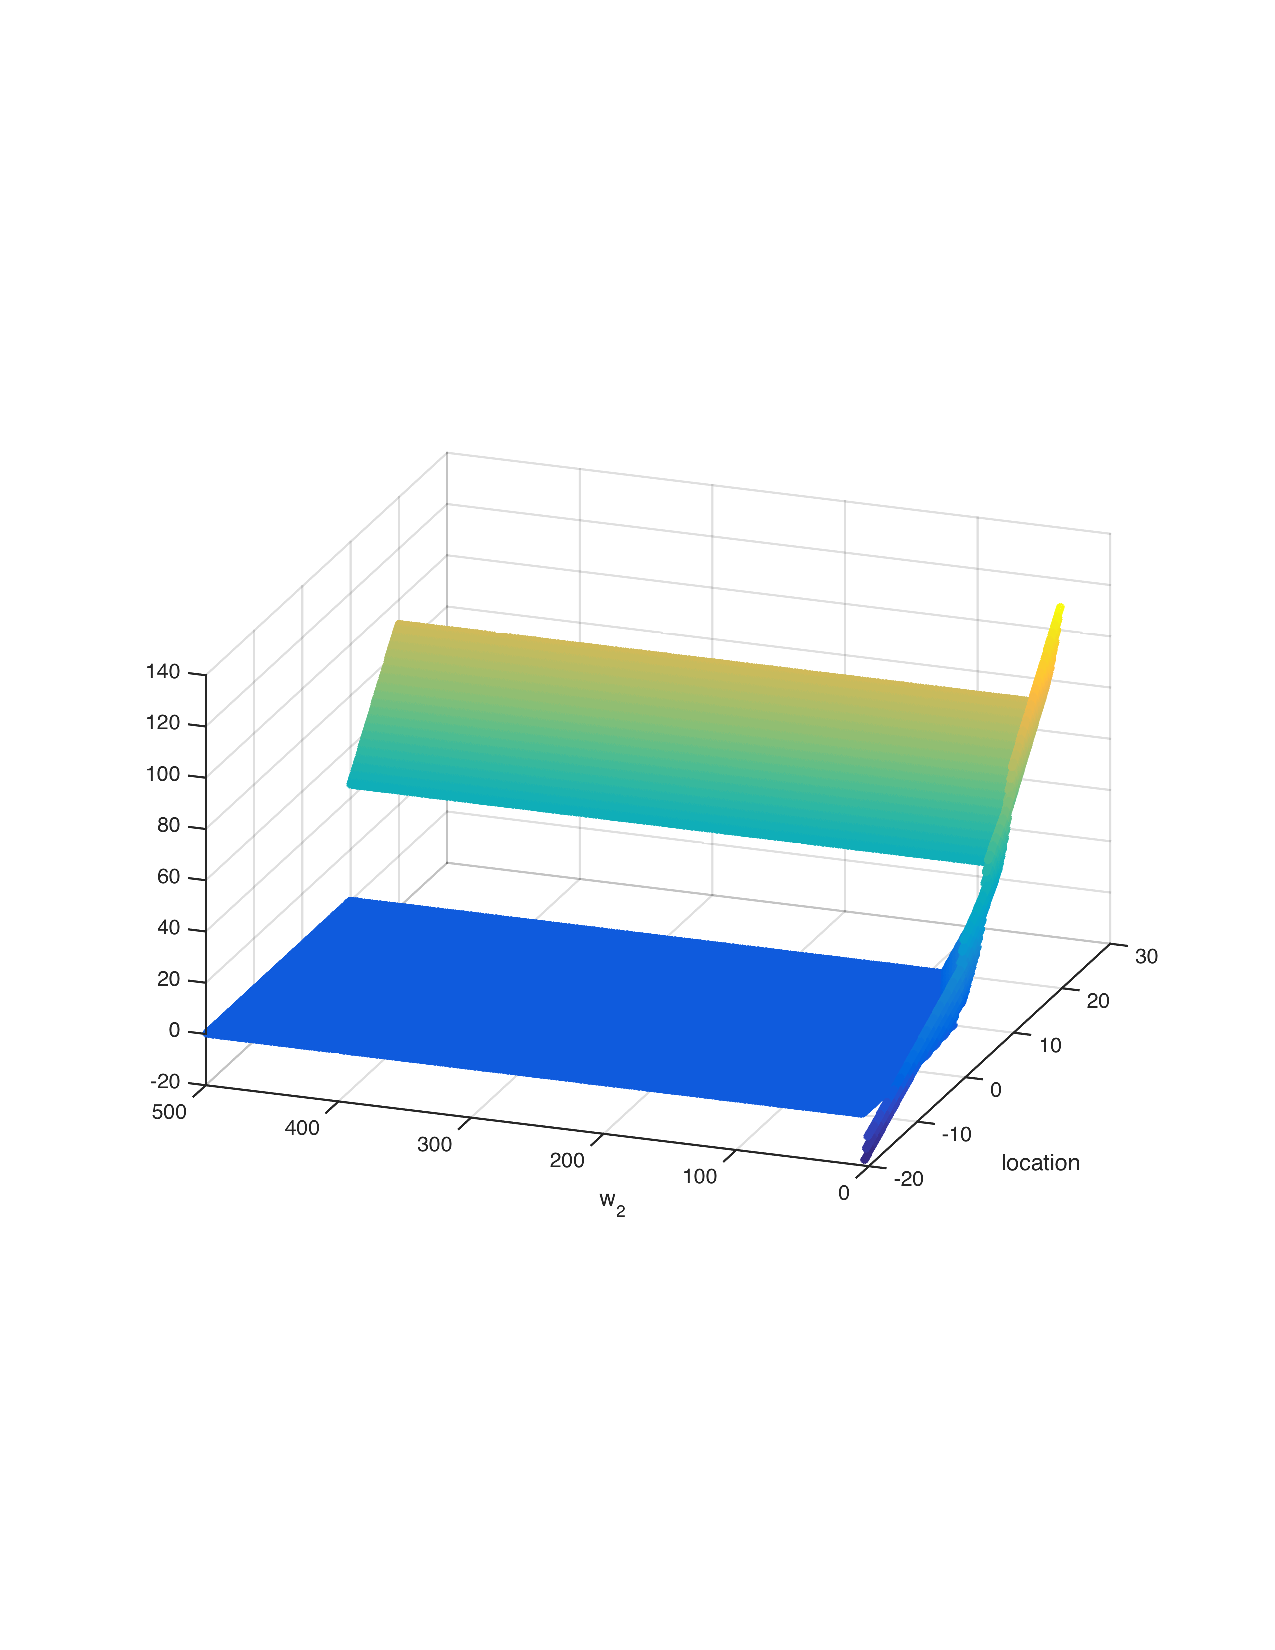
\includegraphics[width=0.9\linewidth, height=0.8\linewidth]{images/robot1d}
    \caption{The Optimal $ \Horizon = 10 $ Value Function for 1-Dimensional Robot. $ \mathtt{threshold} $ was set to 10.0 and $ cost_{\mathtt{movement}} $ was set to -1.0. The x-axis shows $ location \in \left[ -20.0, 20.0 \right]$ and the y-axis shows $ w_2 \in \left[ 0.0, 500.0 \right]$. }
    \label{fig:robot1d}
\end{figure}
%------------------------------------------------------------------------------

\subsection{Influenza Epidemiology Suspectible-Death}
\label{sec:results_sd}

\begin{align*}
    s_{t + 1} &= - s_t \cdot ( \eta + a ) \\
    d_{t+1} &= \eta \cdot s_t 
\end{align*}

where {\footnotesize $ \eta \in [0, 1]$} is the rate of infection and {\footnotesize $ a_t \in \left\lbrace 0, \ldots, 1.0\right\rbrace $} is the proportion of susceptibles {\footnotesize $ s_t $} to be vaccinated. The SD model can be formulated as an MOMDP as follows:

\begin{itemize}
    \item {\footnotesize $ \State = \left\langle S, D \right\rangle$ }, where $ s $ and $ d $ are as defined above
    \item {\footnotesize $ \Action \in \left\lbrace 0, 0.25, 0.50, 1.0 \right\rbrace $} is the proportion of $ S $ to vaccinate
    \item The transition function {\footnotesize \Transition} for each state variable in {\footnotesize \State} is given by:    \\
    {\footnotesize 
        \abovedisplayskip=5pt
        \belowdisplayskip=0pt
        \renewcommand{\arraystretch}{1.5}
        \begin{tabular}{ll}
            $ \Transition\left( s' | s, d, a \right) =$ & $ \delta \left[ s' - (- s \cdot (\eta + a)) \right] $ \\
            $ \Transition\left( d' | s, d, a \right) =$ & $ \delta \left[ d' - (\eta \cdot s) \right] $ \\
        \end{tabular}
    }%
    \item {\footnotesize $ \Reward\left(\vec{w}, cost_{\mathtt{death}}, cost_{\mathtt{vaccine}}, s, d, a \right) = w_1 \cdot \Reward_{\mathtt{death}} + w_2 \cdot \Reward_{\mathtt{vaccine}}$} where, \\
    {\footnotesize 
        \abovedisplayskip=10pt
        \belowdisplayskip=0pt
        \renewcommand{\arraystretch}{1.5}
        \begin{tabular}{ll}    
            $ \Reward_{\mathtt{death}}(s', d', a, cost_{\mathtt{death}}) = $ &  $ $ \\
                \qquad $ \begin{cases}
                (d \geq 0) : & cost_{\mathtt{death}} \cdot d \\
                \text{otherwise} : & 0 \\
                \end{cases} $ & $ $ \\
            $ \Reward_{\mathtt{vaccine}}(s', d', a, cost_{\mathtt{vaccine}}) = $ &  $ $ \\
                \qquad $ \begin{cases}
                (s \geq 0) : & cost_{\mathtt{vaccine}} \cdot s \cdot a \\
                \text{otherwise} : & 0 \\
                \end{cases} $ & $ $ \\
        \end{tabular}
    }    
\end{itemize} 

%------------------------------------------------------------------------------
% Figure
\begin{figure}[t!]
    \centering
    \begin{subfigure}[b]{0.4\textwidth}
%        \centering
        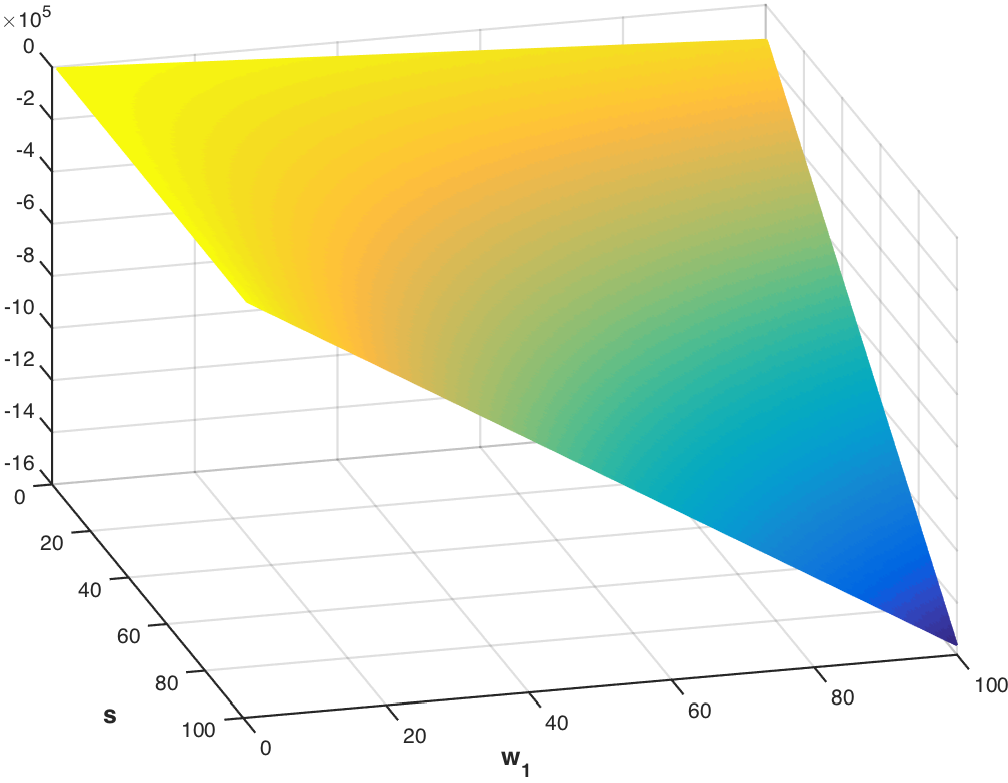
\includegraphics[width=\linewidth, height=0.8\linewidth]{images/sd_w1}
        \caption{$ w_1 \in \left[ 0.0, 100.0 \right]$}
        \label{fig:opt_execution_w1}
        \vspace{1em}
    \end{subfigure}
    
    \begin{subfigure}[b]{0.4\textwidth}
%        \centering
        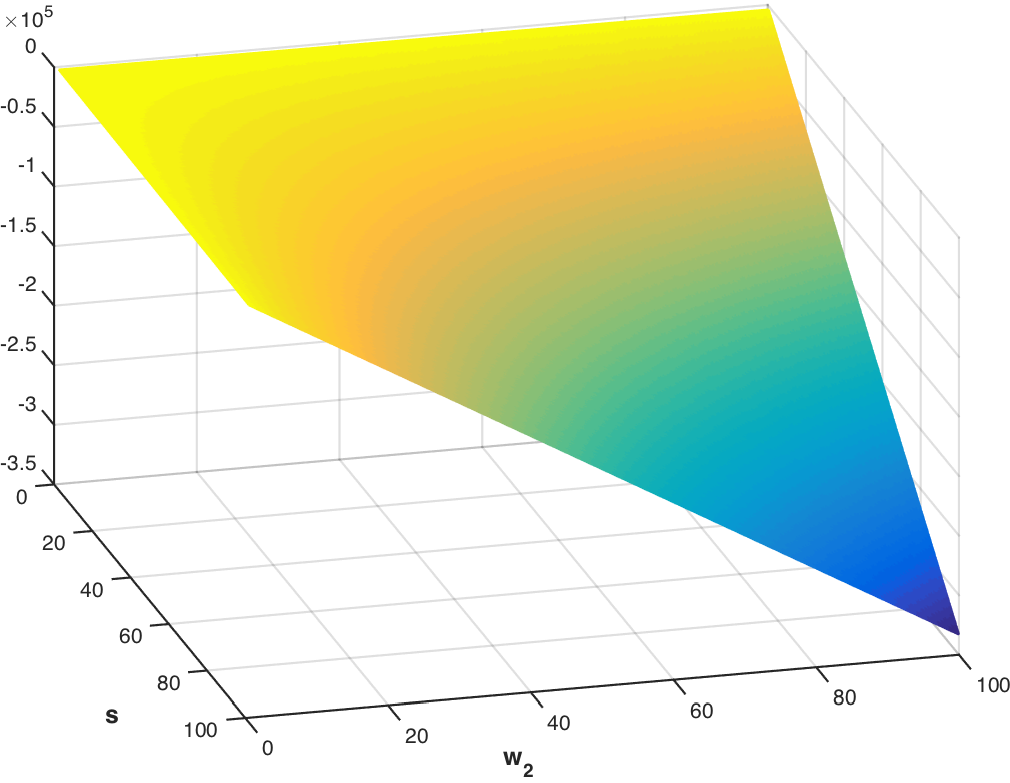
\includegraphics[width=\linewidth, height=0.8\linewidth]{images/sd_w2}
        \caption{$ w_2 \in \left[ 0.0, 100.0 \right]$}
        \label{fig:pt_execution_w2}
    \end{subfigure}  
    \caption{Influenza S-D Epidemiology. $ \eta = 0.0165, d = 1.0, cost_{\mathtt{death}} = 95.0, cost_{\mathtt{vaccine}} = 33.0$.}
    \label{fig:pt_execution}
\end{figure}
%------------------------------------------------------------------------------

\subsection{Influenza Epidemiology Susceptible-Infected-Recovered-Susceptible}
\label{sec:results_ee}

We can describe Influenza epidemics by an SIRS (Susceptible-Infective-Recovered-Susceptible) model. {\footnotesize $ S $} refer to the number of susceptibles, {\footnotesize $ I $} to number of infected and {\footnotesize $ R $} to the recovered. At each time step the population in each of the three populations is updated according to the following equations:
\begin{align*}
    s_{t + 1} &= -\eta \cdot s_t \cdot i_t + c \cdot r_t - a_t \cdot s_t \\
    i_{t + 1} &= \eta \cdot s_t \cdot i_t - b \cdot i_t \\
    r_{t+1} &= b \cdot i_t - c \cdot r_t 
%    d_{t+1} &= e \cdot i_t 
\end{align*}

where {\footnotesize $ \eta \in [0, 1]$} is the rate of infection, {\footnotesize $ b \in [0, 1]$} is the rate of recovery and {\footnotesize $ c \in [0, 1]$} is the rate of susceptibility. At each decision epoch we allow a proportion of susceptibles {\footnotesize $ s_t $} to be immunised i.e. {\footnotesize $ a_t \in \left\lbrace 0, \ldots, 1.0\right\rbrace $}. The Influenza SIR model can be formulated as an MOMDP as follows:

\begin{itemize}
    \item {\footnotesize $ \State = \left\langle S, I, R \right\rangle$ }, where $ S $, $ I $, and $ R $ are as defined above
    \item {\footnotesize $ \Action \in \left\lbrace 0, 0.25, 0.50, 1.0 \right\rbrace $} is the proportion of $ S $ to vaccinate
%\end{itemize}
%\begin{itemize}
    \item The transition function {\footnotesize \Transition} for each state variable in {\footnotesize \State} is given by:    
    {\footnotesize 
        \abovedisplayskip=5pt
        \belowdisplayskip=0pt
        \renewcommand{\arraystretch}{1.5}
        \begin{tabular}{ll}
            $ \Transition\left( s' | s, i, r, a \right) =$ & $ \delta \left[ s' - (- \eta \cdot s \cdot i + c \cdot r -a \cdot s) \right] $ \\
            $ \Transition\left( i' | s, i, r, a \right) =$ & $ \delta \left[ i' - (\eta \cdot s \cdot i - b \cdot i) \right] $ \\
            $ \Transition\left( r' | s, i, r, a \right) =$ & $ \delta \left[ r' - (b \cdot i - c \cdot r) \right] $ \\            
        \end{tabular}
    }%
    \item {\footnotesize $ \Reward\left(\vec{w}, cost_{\mathtt{inf}}, s, i, r, a \right) = w_1 \cdot -cost_{\mathtt{inf}} \cdot i + w_2 \cdot -cost_{\mathtt{vaccine}} \cdot a $}, where {\footnotesize $ cost_{\mathtt{inf}} $} is the incident cost of infection and {\footnotesize $ cost_{\mathtt{vaccine}} $} is the unit cost of vaccination \\
\end{itemize} 

%------------------------------------------------------------------------------
% Figure
\begin{figure}[t!]
    \centering
    \begin{subfigure}[b]{0.4\textwidth}
        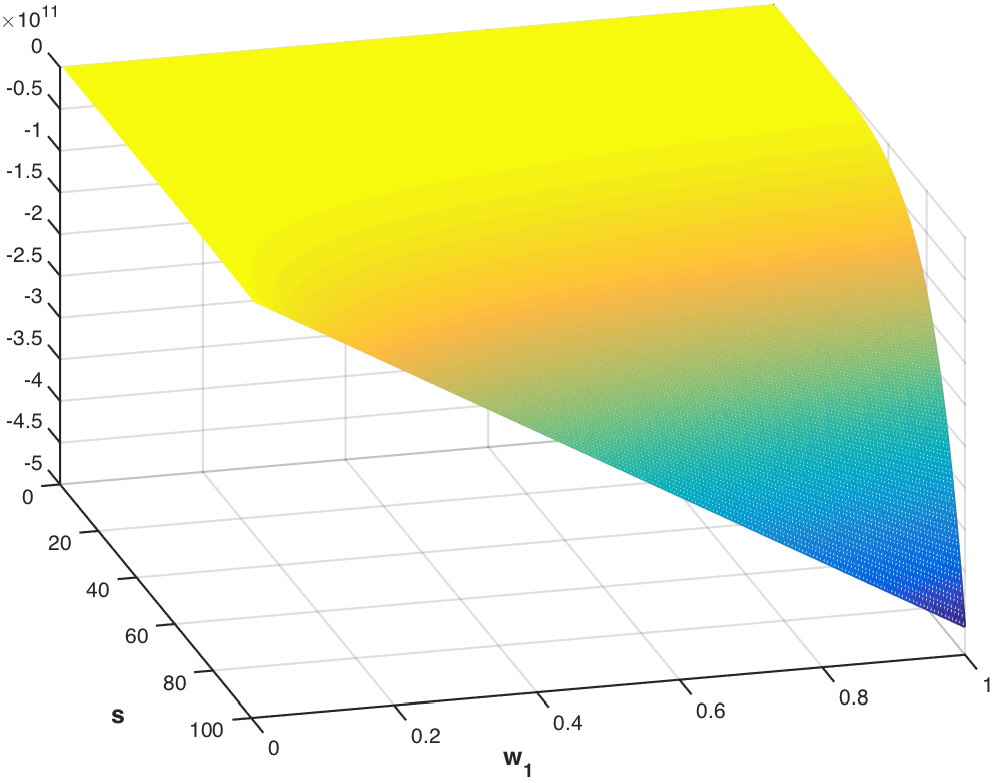
\includegraphics[width=\linewidth, height=0.8\linewidth]{images/sir_s_w1}
        \caption{$ s \in \left[ 0.0, 100.0 \right], w_1 \in \left[ 0.0, 100.0 \right], i = 50.0, r = 50.0$}
        \label{fig:sir_s_w1}
        \vspace{1em}
    \end{subfigure}
    
    \begin{subfigure}[b]{0.4\textwidth}
        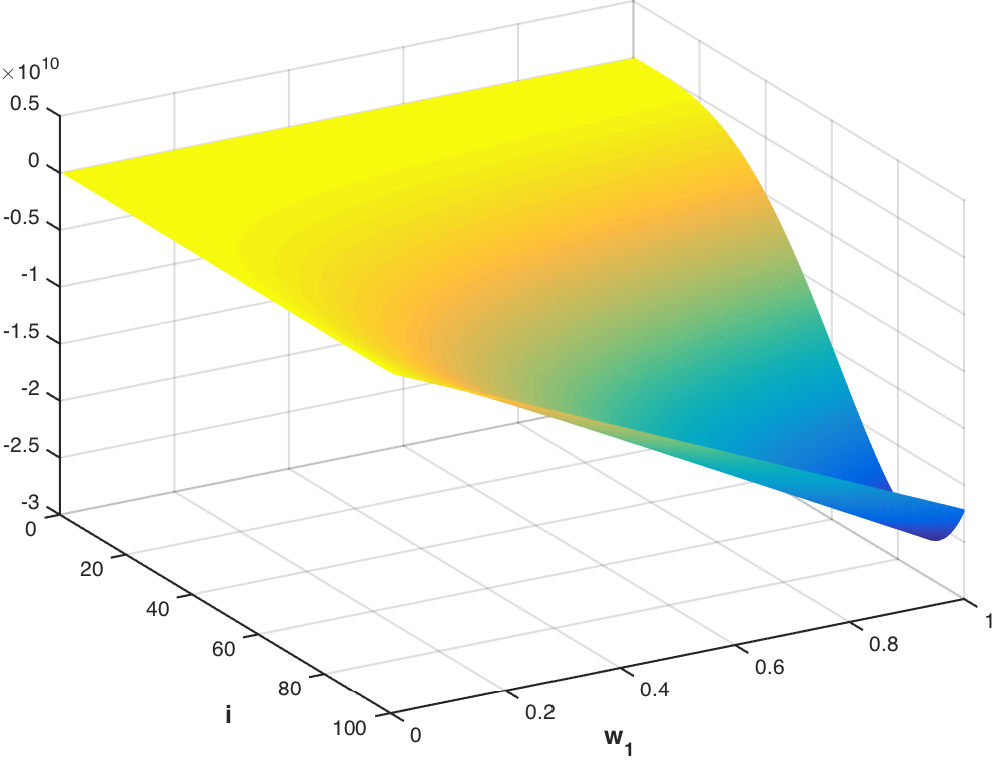
\includegraphics[width=\linewidth, height=0.8\linewidth]{images/sir_i_w1}
        \caption{$ i \in \left[ 0.0, 100.0 \right],w_1 \in \left[ 0.0, 100.0 \right], s = 50.0, r = 50.0$}
        \label{fig:sir_i_w1}
    \end{subfigure}  
    
    \begin{subfigure}[b]{0.4\textwidth}
        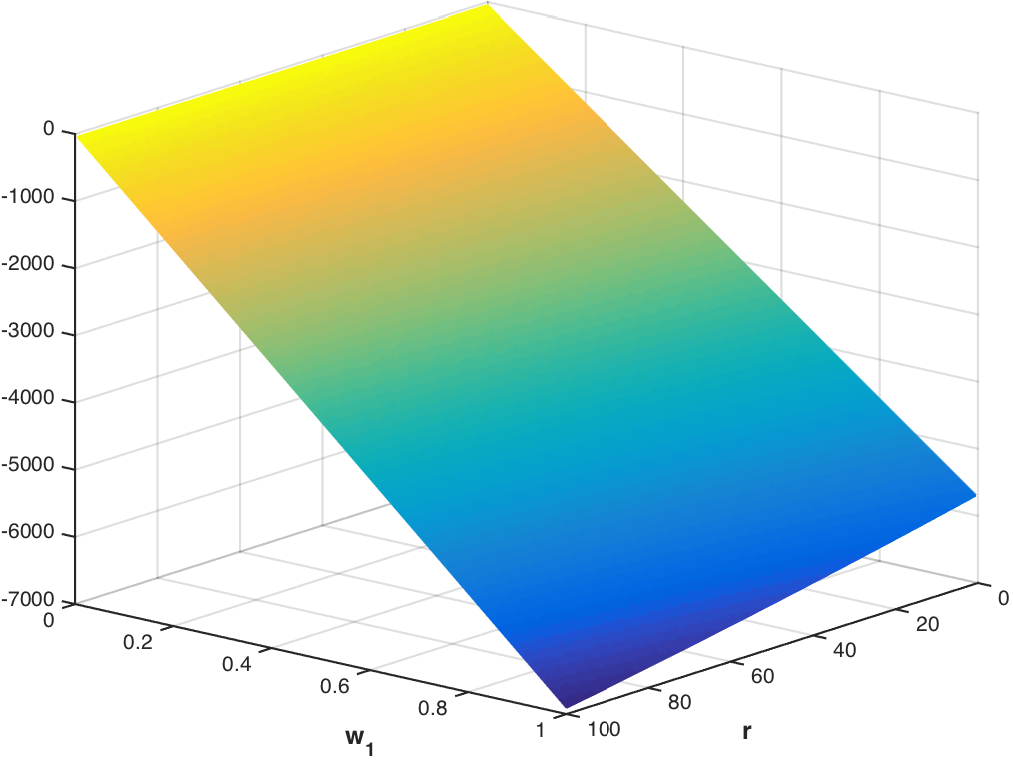
\includegraphics[width=\linewidth, height=0.8\linewidth]{images/sir_r_w1}
        \caption{$ r \in \left[ 0.0, 100.0 \right], w_1 \in \left[ 0.0, 100.0 \right], s = 50.0, i = 50.0$}
        \label{fig:sir_r_w1}
    \end{subfigure}      
    \caption{Influenza S-I-R-S Epidemiology. $ \eta = 1.65 \times 10^2, b = 0.27, c = 0.23, cost_{\mathtt{inf}} = 95.0, cost_{\mathtt{vaccine}} = 33.0$.}
    \label{fig:sir}
\end{figure}
%------------------------------------------------------------------------------
    
%%\begin{figure}[h!]
%%    \centering
%%    \fbox{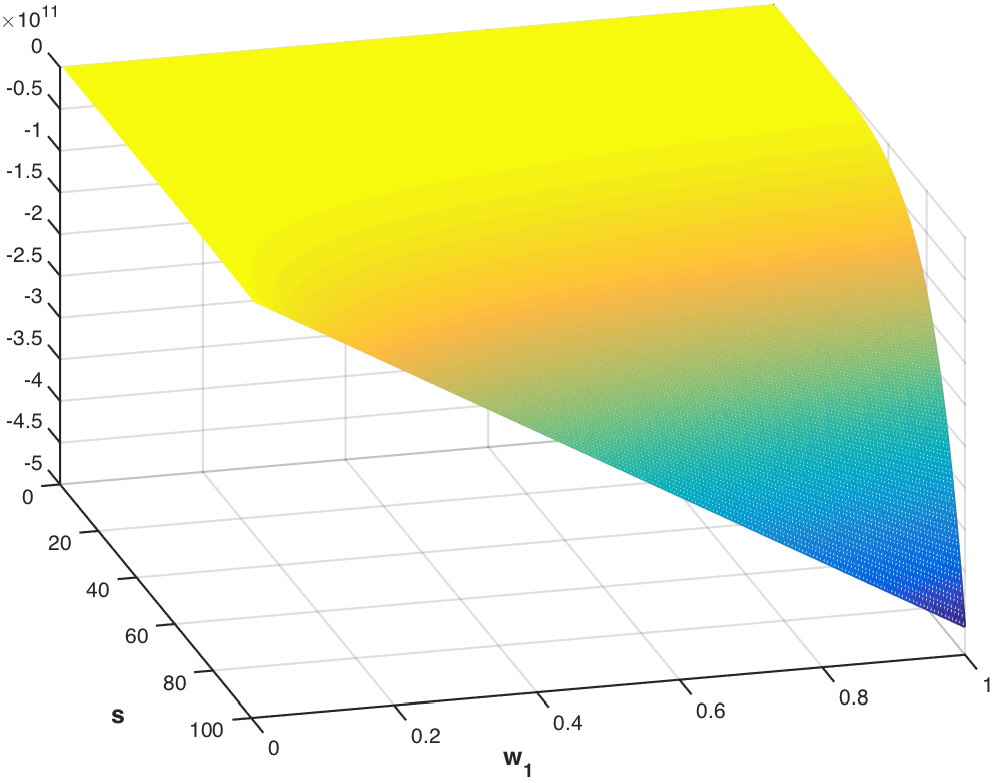
\includegraphics[width=\linewidth]{images/sir_s_w1}}
%%    \caption{Influenza Epidemiology. $ s \in \left[ 0.0, 100.0 \right]$ is on the x-axis and $ w_1 \in \left[ 0.0, 100.0 \right]$ is on the y-axis. $ i = 50.0, r = 50.0 \eta = 1.65 \times 10^2, b = 0.27, c = 0.23, cost_{\mathtt{inf}} = 95.0, cost_{\mathtt{vaccine}} = 33.0$.}
%%    \label{fig:robot1d}
%%\end{figure}
%%
%%\begin{figure}[h!]
%%    \centering
%%    \fbox{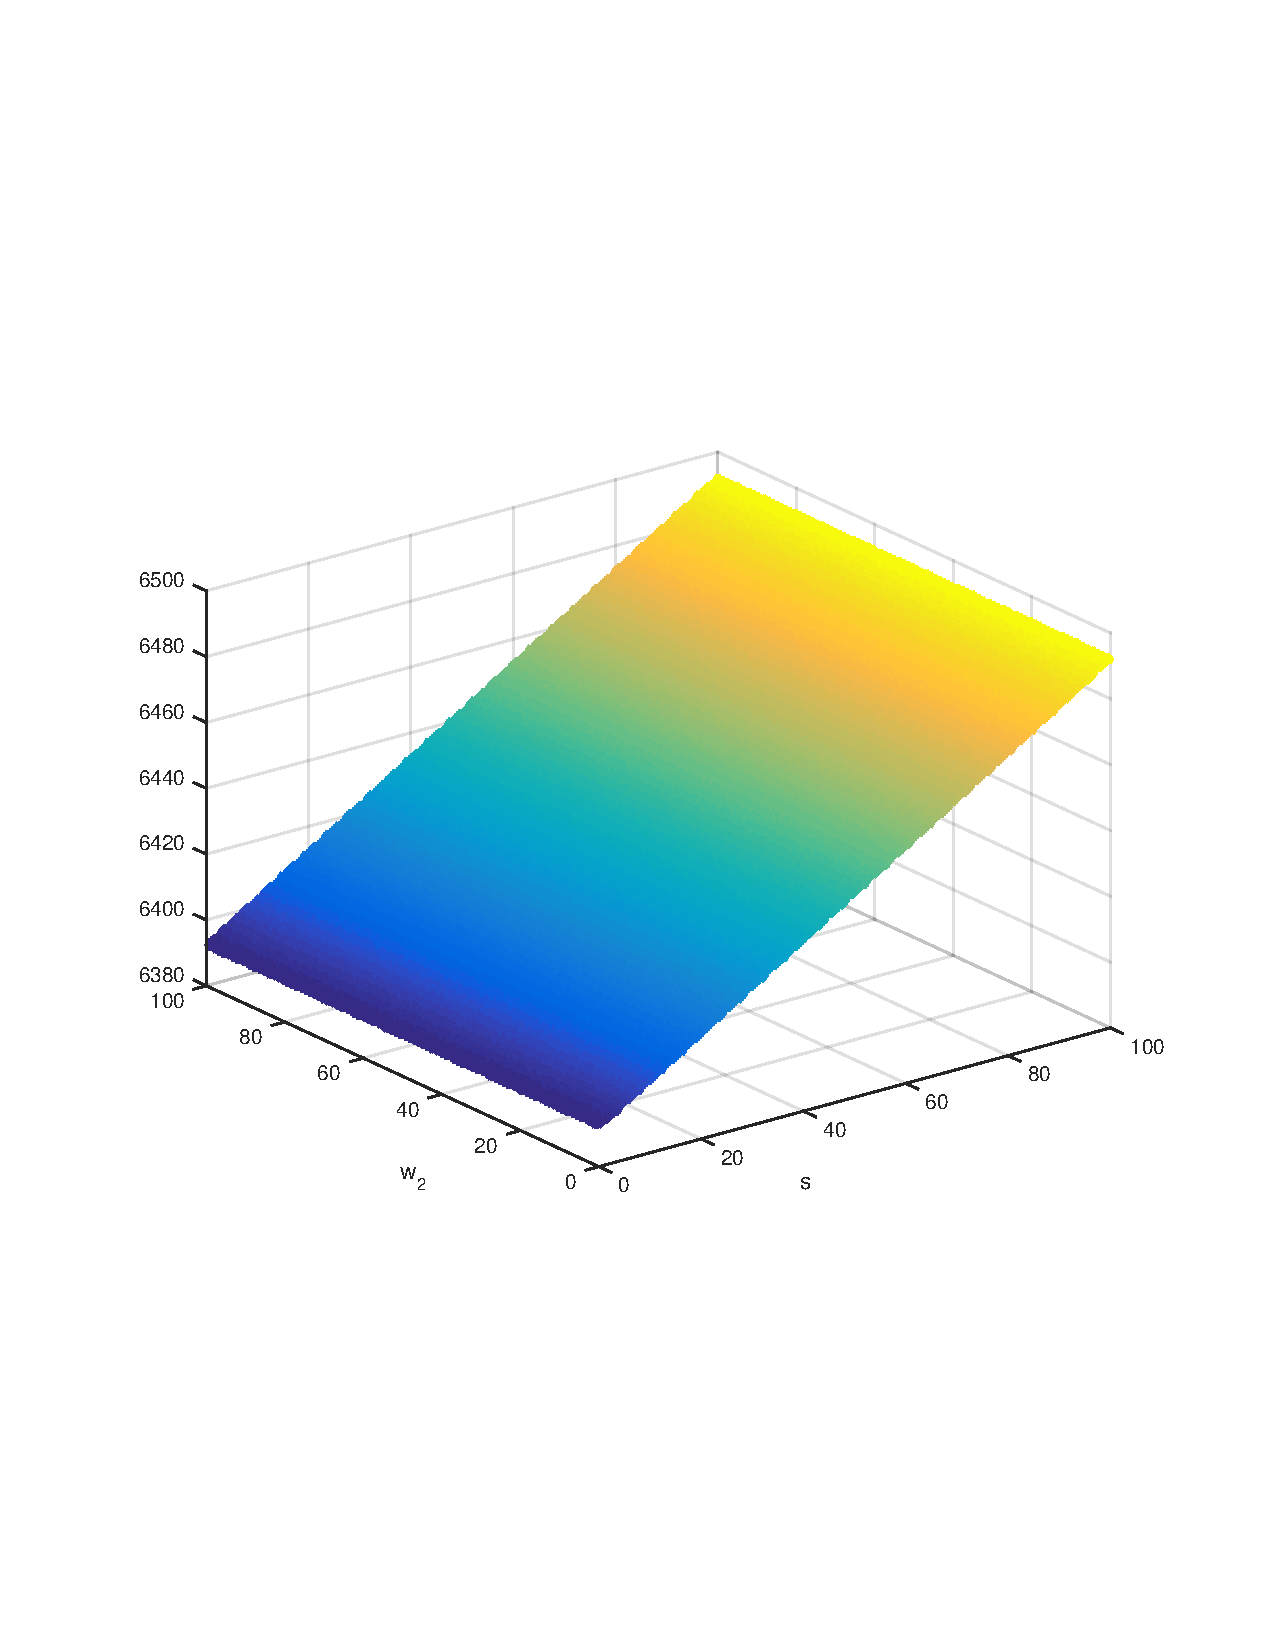
\includegraphics[width=\linewidth]{images/sir_s_w2}}
%%    \caption{Influenza Epidemiology. $ s \in \left[ 0.0, 100.0 \right]$ is on the x-axis and $ w_1 \in \left[ 0.0, 100.0 \right]$ is on the y-axis. $ i = 50.0, r = 50.0 \eta = 1.65 \times 10^2, b = 0.27, c = 0.23, cost_{\mathtt{inf}} = 95.0, cost_{\mathtt{vaccine}} = 33.0$.}
%%    \label{fig:robot1d}
%%\end{figure}
%%
%%\begin{figure}[h!]
%%    \centering
%%    \fbox{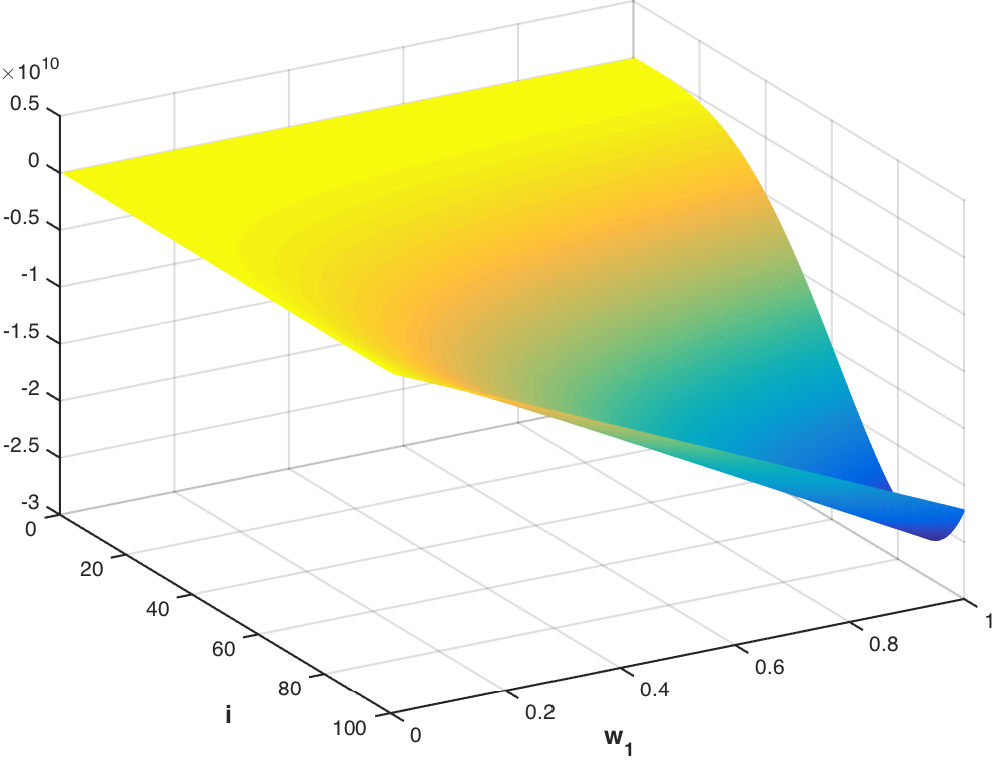
\includegraphics[width=\linewidth]{images/sir_i_w1}}
%%    \caption{Influenza Epidemiology. $ i \in \left[ 0.0, 100.0 \right]$ is on the x-axis and $ w_1 \in \left[ 0.0, 100.0 \right]$ is on the y-axis. $ s = 50.0, r = 50.0 \eta = 1.65 \times 10^2, b = 0.27, c = 0.23, cost_{\mathtt{inf}} = 95.0, cost_{\mathtt{vaccine}} = 33.0$.}
%%    \label{fig:robot1d}
%%\end{figure}
%%
%%\begin{figure}[h!]
%%    \centering
%%    \fbox{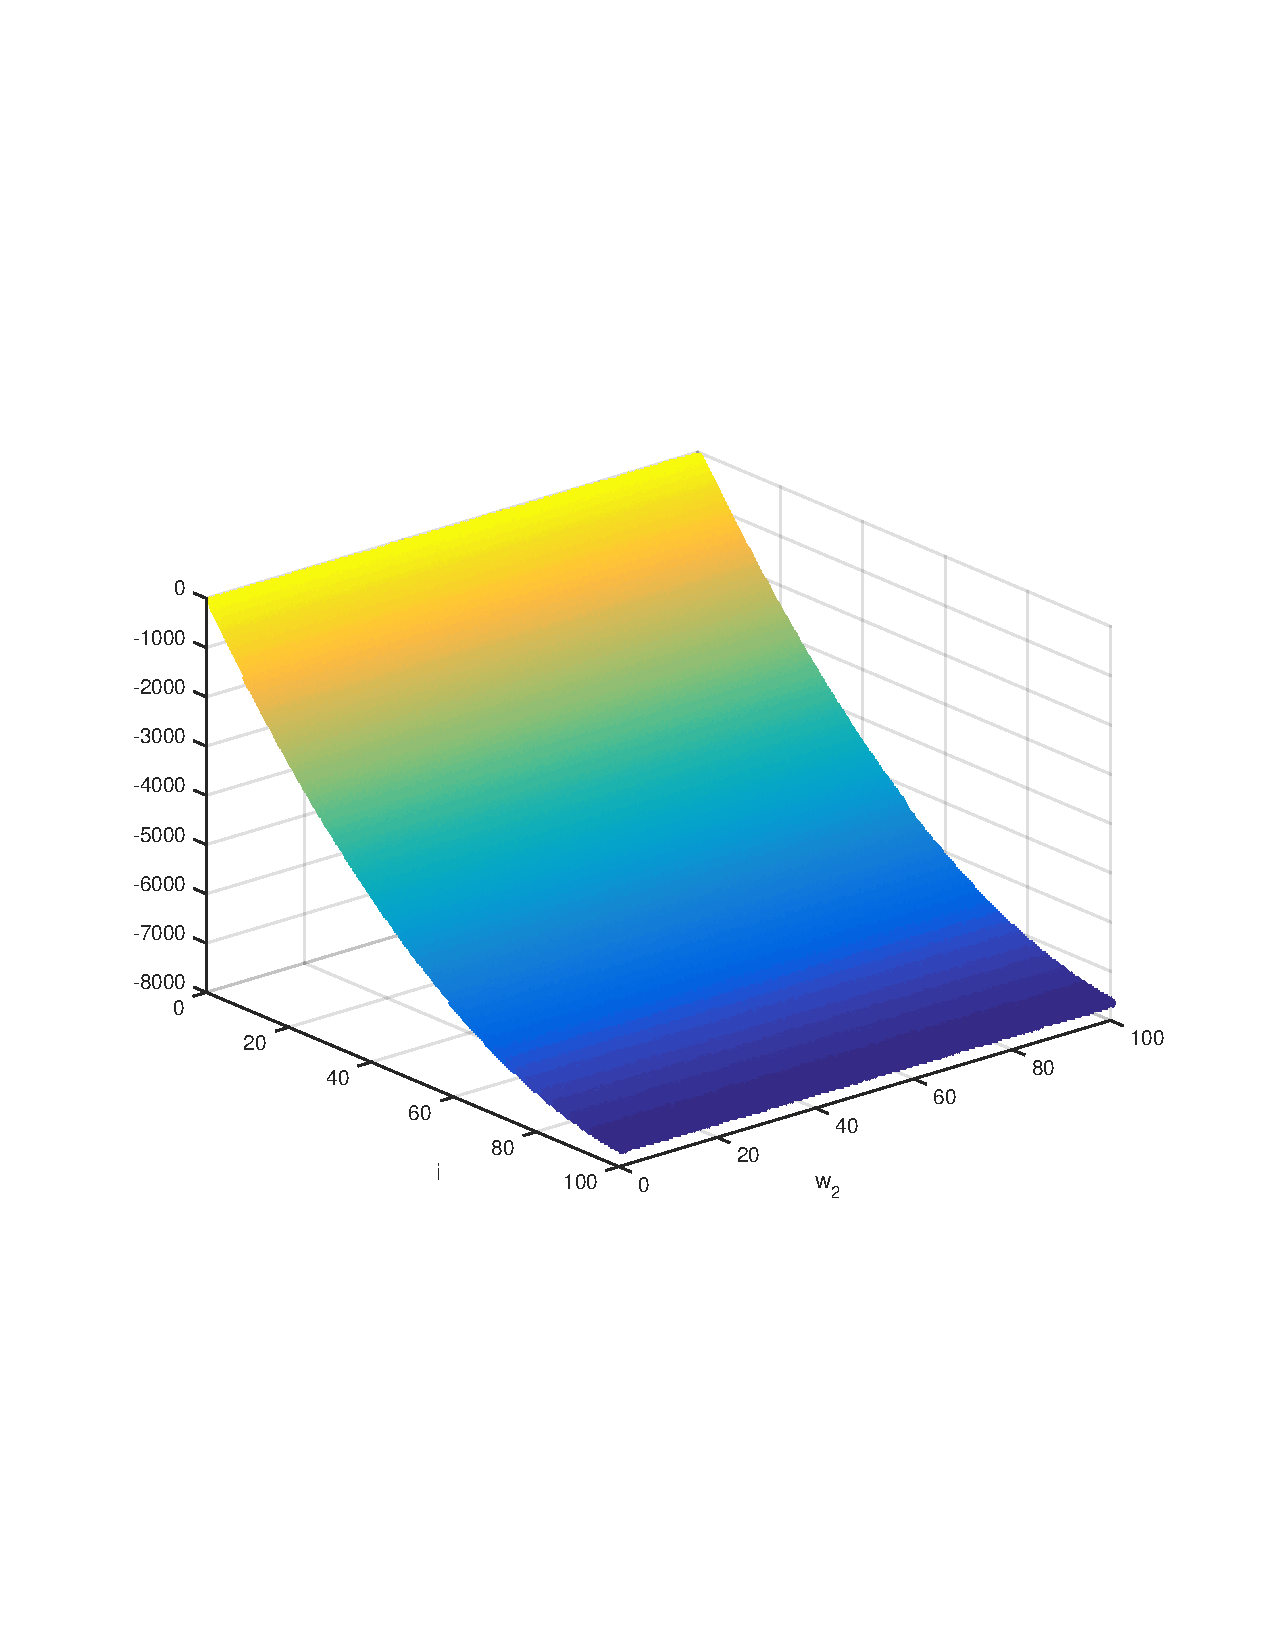
\includegraphics[width=\linewidth]{images/sir_i_w2}}
%%    \caption{Influenza Epidemiology. $ i \in \left[ 0.0, 100.0 \right]$ is on the x-axis and $ w_1 \in \left[ 0.0, 100.0 \right]$ is on the y-axis. $ s = 50.0, r = 50.0 \eta = 1.65 \times 10^2, b = 0.27, c = 0.23, cost_{\mathtt{inf}} = 95.0, cost_{\mathtt{vaccine}} = 33.0$.}
%%    \label{fig:robot1d}
%%\end{figure}
%%
%%\begin{figure}[h!]
%%    \centering
%%    \fbox{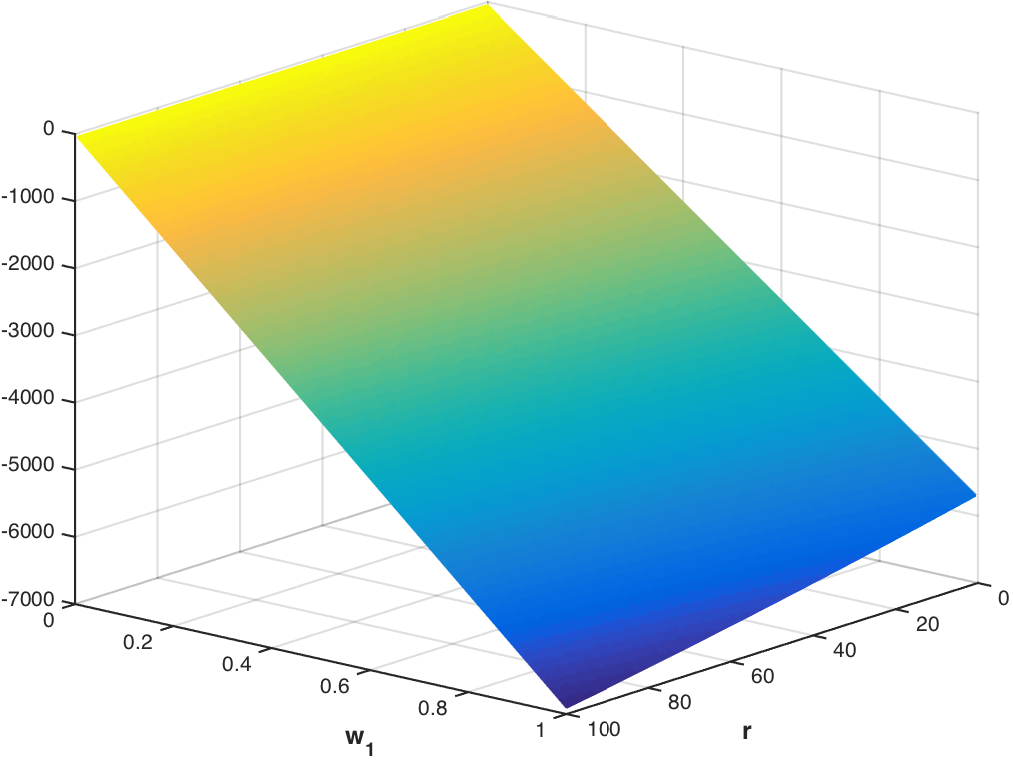
\includegraphics[width=\linewidth]{images/sir_r_w1}}
%%    \caption{Influenza Epidemiology. $ r \in \left[ 0.0, 100.0 \right]$ is on the x-axis and $ w_1 \in \left[ 0.0, 100.0 \right]$ is on the y-axis. $ s = 50.0, i = 50.0 \eta = 1.65 \times 10^2, b = 0.27, c = 0.23, cost_{\mathtt{inf}} = 95.0, cost_{\mathtt{vaccine}} = 33.0$.}
%%    \label{fig:robot1d}
%%\end{figure}
%%
%%\begin{figure}[h!]
%%    \centering
%%    \fbox{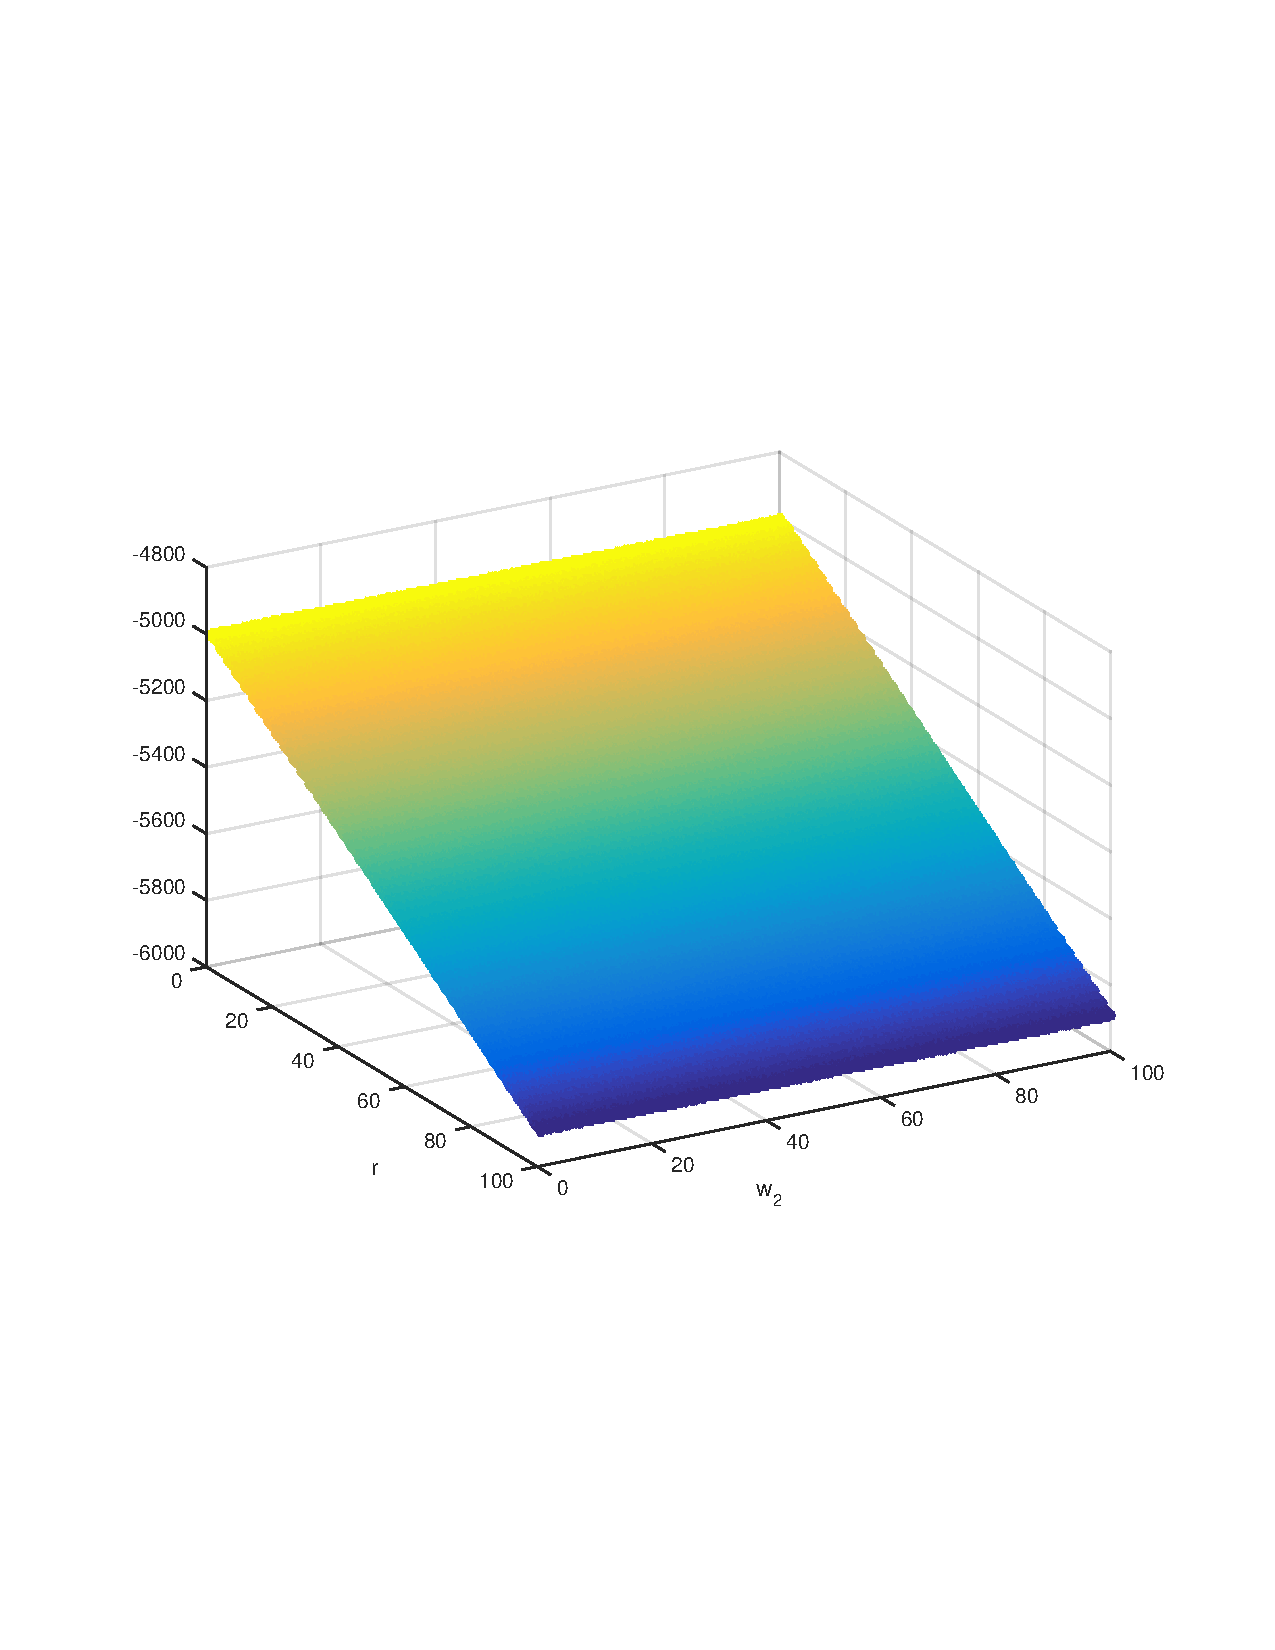
\includegraphics[width=\linewidth]{images/sir_r_w2}}
%%    \caption{Influenza Epidemiology. $ r \in \left[ 0.0, 100.0 \right]$ is on the x-axis and $ w_1 \in \left[ 0.0, 100.0 \right]$ is on the y-axis. $ s = 50.0, i = 50.0 \eta = 1.65 \times 10^2, b = 0.27, c = 0.23, cost_{\mathtt{inf}} = 95.0, cost_{\mathtt{vaccine}} = 33.0$.}
%%    \label{fig:robot1d}
%%\end{figure}
%%
%%\begin{figure}[h!]
%%    \centering
%%    \fbox{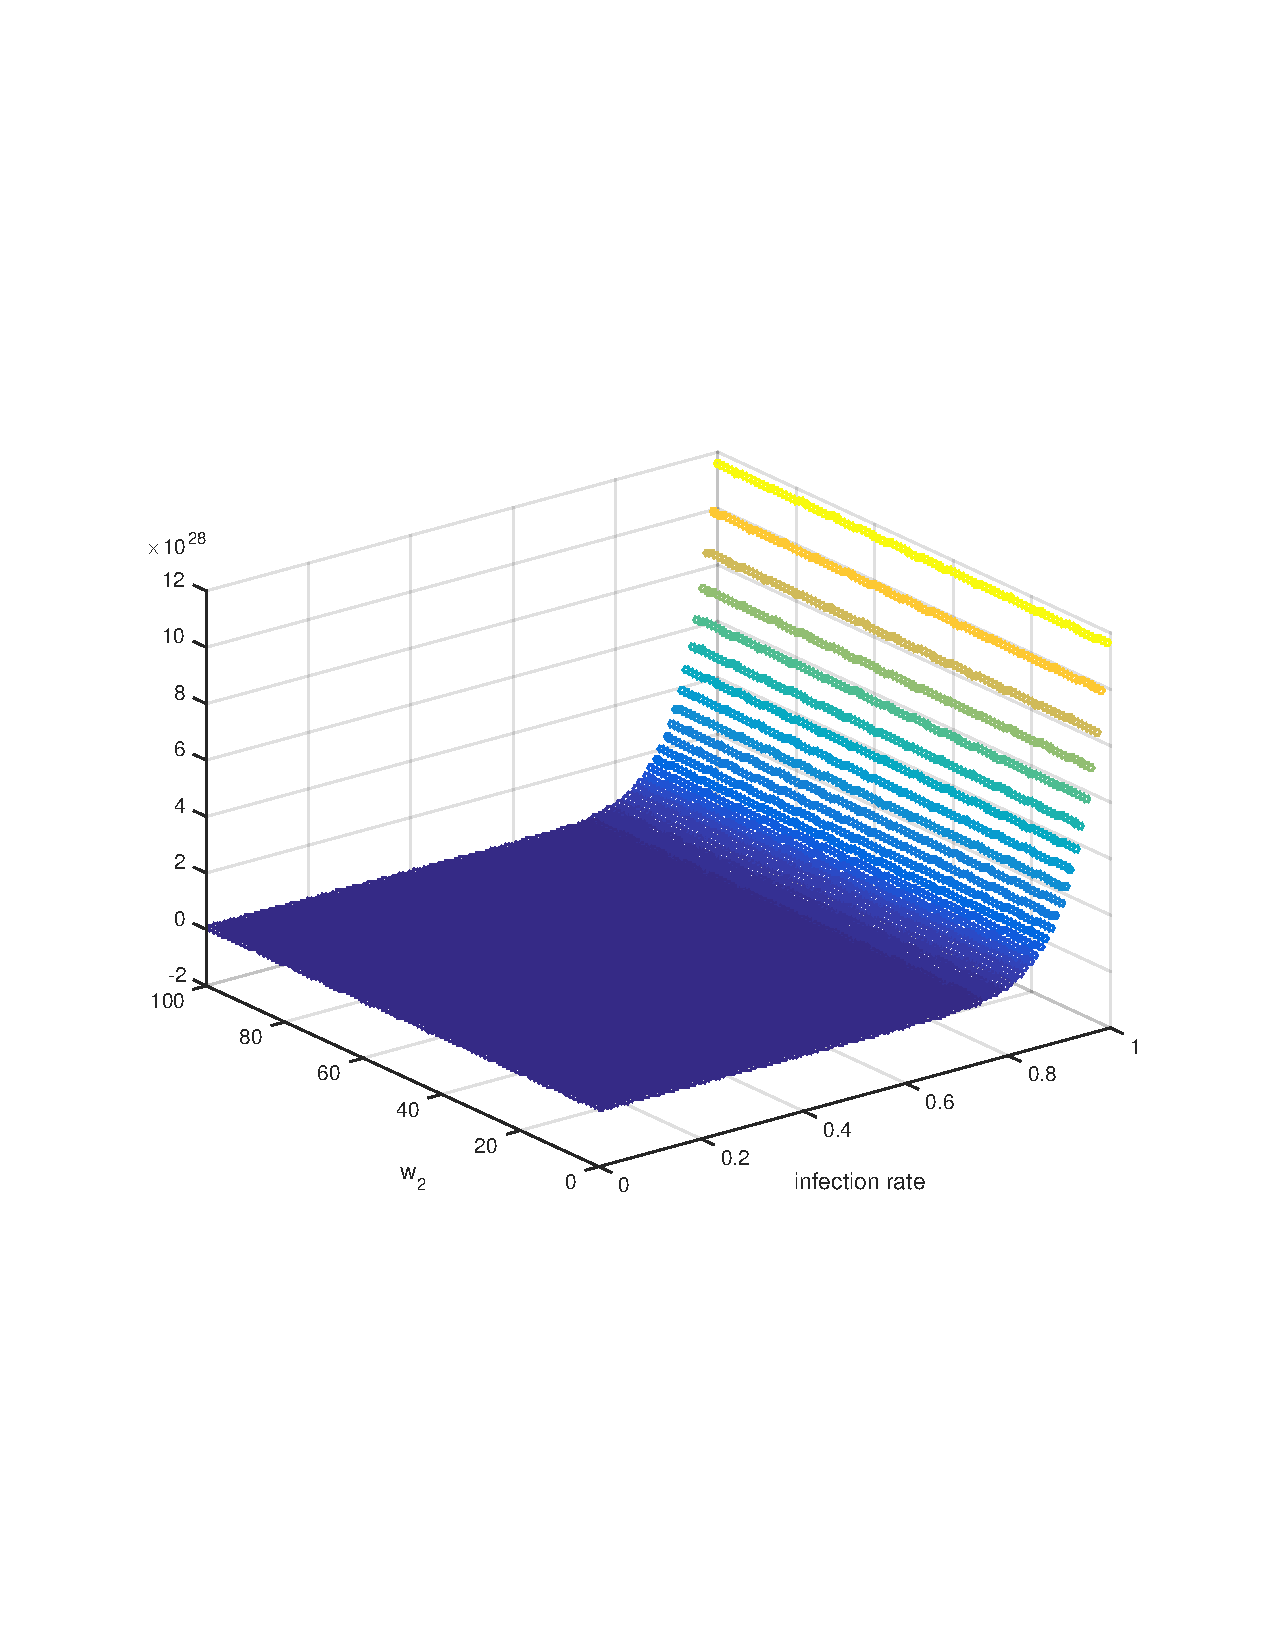
\includegraphics[width=\linewidth]{images/sir_infection_w2}}
%%    \caption{Influenza Epidemiology. $ \eta \in \left[ 0.0, 1.0 \right]$ is on the x-axis and $ w_2 \in \left[ 0.0, 100.0 \right]$ is on the y-axis. $ s = 50.0, i = 50.0, r = 50.0, b = 0.27, c = 0.23, cost_{\mathtt{inf}} = 95.0, cost_{\mathtt{vaccine}} = 33.0$.}
%%    \label{fig:robot1d}
%%\end{figure}
%
%%\subsection{Automated Market Making}
%%\label{sec:results_mm}
%%
%%\begin{itemize}
%%    \item {\footnotesize $\State = \left\langle i, v\right\rangle$}, where {\footnotesize $v \in \Real^{+}$} is the value of the asset and {\footnotesize $i \in \Natural$} represents the MM's inventory.
%%    \item {\footnotesize $\Action = \left\lbrace \left(bid_1, ask_1\right), \ldots,
%%        \left(bid_N, ask_N\right) \right\rbrace$} represents a finite set of allowed $N$ bid-ask pairs, where {\footnotesize $bid_n, ask_n \in \Real^{+}$} and {\footnotesize $bid_n < ask_n$}. 
%%\end{itemize}      
%%
%%The \bid represents the price at which the MM is willing to buy one unit of the asset and the \ask is the price at which the MM is willing to sell one unit of the asset.
%%
%%\begin{itemize}
%%    \item The transition function {\footnotesize \Transition} for each state variable in {\footnotesize \State} is given by: \\   
%%    {\footnotesize 
%%        \abovedisplayskip=5pt
%%        \belowdisplayskip=0pt
%%        \renewcommand{\arraystretch}{1.5}
%%        \begin{tabular}{ll}
%%            $ \Transition\left( i' | i, v, bid, ask \right) =$ & $ \delta \left[ i' - \begin{cases}
%%            v > ask  \wedge (i \geq 1) : & i - 1 \\
%%            v < bid  : & i + 1 \\
%%            \text{otherwise} : & i \\
%%            \end{cases} \right] $ \\
%%            $ \Transition\left( v' | i, v, bid, ask \right) =$ & $ \delta \left[ v' - v \right] $ \\
%%        \end{tabular}
%%    }%
%%    \item The reward function {\footnotesize \Reward}, is specified as {\footnotesize $ \Reward\left(\vec{w}, i, n \right) = w_1 \cdot \Reward_{\mathtt{profit}} + w_2 \cdot \Reward_{\mathtt{liquidity}} $} where, \\
%%    {\footnotesize 
%%        \abovedisplayskip=10pt
%%        \belowdisplayskip=0pt
%%        \renewcommand{\arraystretch}{1.5}
%%        \begin{tabular}{ll}    
%%            $ \Reward_{\mathtt{profit}}(i', v', bid, ask) = $ & $ $ \\
%%            \qquad $ \begin{cases}
%%            (v' > ask) \wedge (i' \geq 1) : & ask \\
%%            (v' < bid) : & -bid \\
%%            (v' > bid) \wedge (v' < ask) : & 0 \\
%%            (v' > ask) \wedge (i' < 0) : & 0 \\
%%            \text{otherwise} : & -\infty \\
%%            \end{cases} $ & $ $ \\
%%            $ \Reward_{\mathtt{liquidity}}(i', v', bid, ask) = $ & $ $ \\
%%            \qquad $ \begin{cases}
%%            ask - bid \leq k : & k - (ask - bid) \\
%%            \text{otherwise} : & -\infty \\ 
%%            \end{cases} $ & $ $ \\
%%        \end{tabular}
%%    }    
%%\end{itemize}
%%
%%The MM aims to maximise profit via {\footnotesize $ \Reward_{\mathtt{profit}} $} and market quality via {\footnotesize $ \Reward_{\mathtt{liquidity}} $}.
%%
%%\begin{figure}[h!]
%%    \centering
%%    \fbox{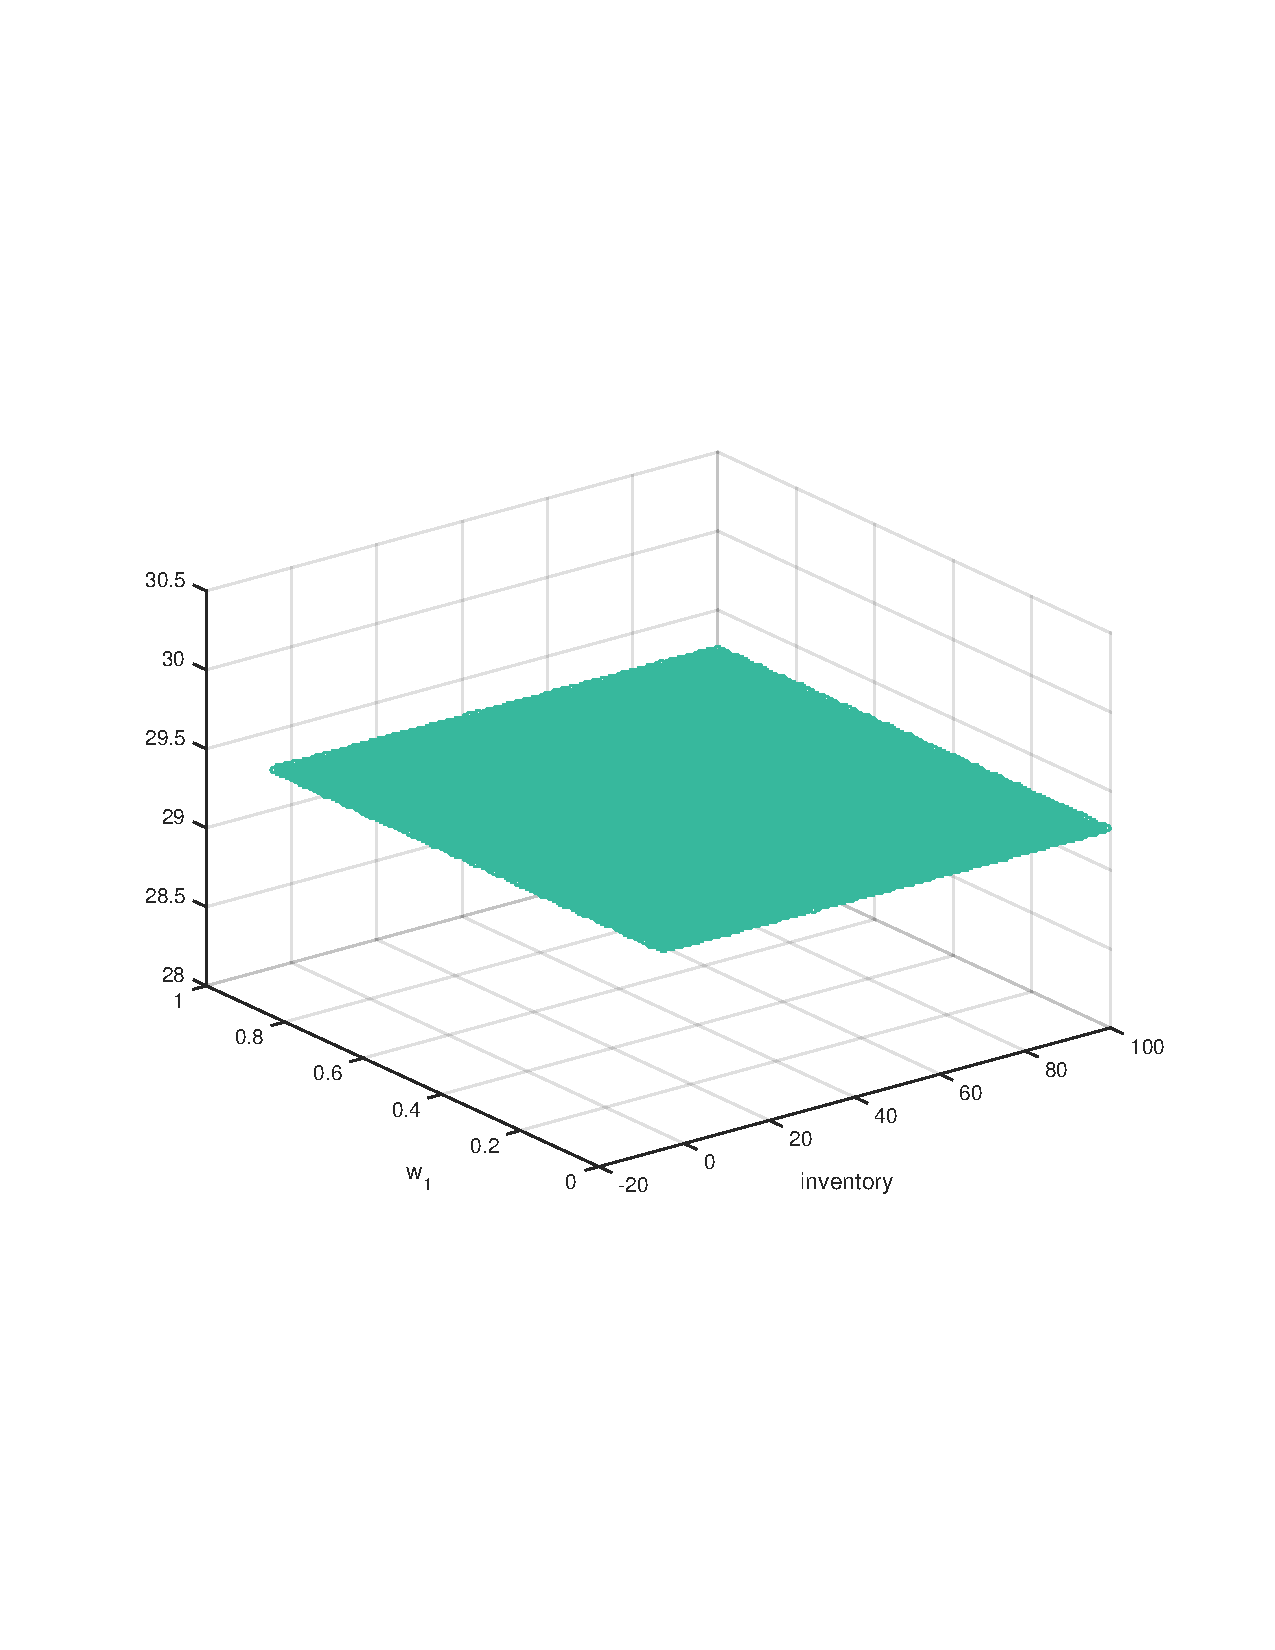
\includegraphics[width=\linewidth]{images/market_making_i_w1}}
%%    \caption{Market Making. $ i \in \left[ -5.0, 100.0 \right]$ is on the x-axis and $ w_1 \in \left[ 0.0, 1.0 \right]$ is on the y-axis. $ v = 50.0, k = 25.0$ and $w_2 = 1.0.$}
%%    \label{fig:robot1d}
%%\end{figure}
%%
%%\begin{figure}[h!]
%%    \centering
%%    \fbox{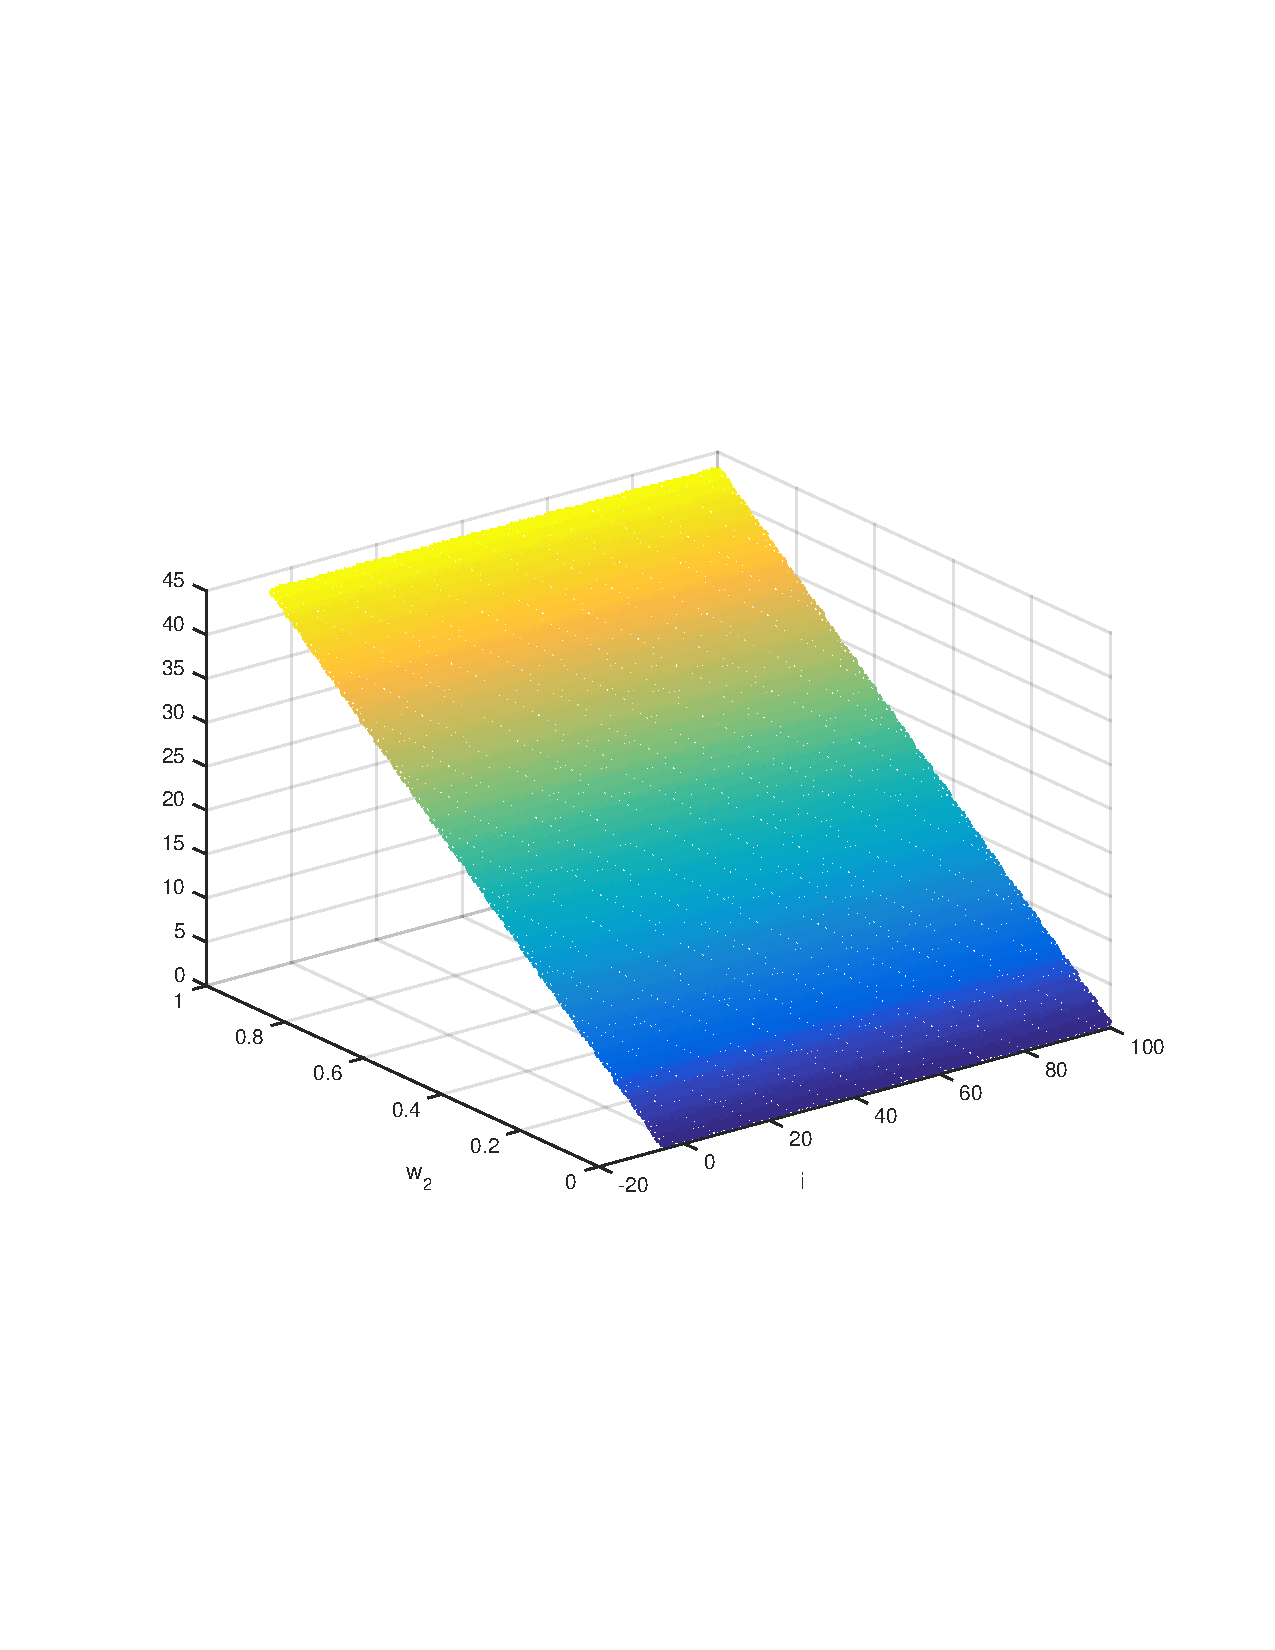
\includegraphics[width=\linewidth]{images/market_making_i_w2}}
%%    \caption{Market Making. $ i \in \left[ -5.0, 100.0 \right]$ is on the x-axis and $ w_2 \in \left[ 0.0, 1.0 \right]$ is on the y-axis. $ v = 50.0, k = 25.0$ and $w_2 = 1.0.$}
%%    \label{fig:robot1d}
%%\end{figure}

\subsection{Optimal Execution}
\label{sec:results_oe}

An investor wishes to buy or sell {\footnotesize $ X \in \mathbb{N} $} shares over {\footnotesize $ [0, T] $}, where {\footnotesize $ X $} and {\footnotesize $ T $} are fixed. Bertsimas and Lo~\parencite{Bertsimas_JFM_1998} formulated a price impact model as:
\begin{align*}
    price_{t+1} &= price_t + \theta \cdot n_{t + 1} + \sigma \cdot \epsilon_{t+1}
\end{align*}

where {\footnotesize $ s_t $ } is the price at the beginning of period {\footnotesize $ t $}, {\footnotesize $\sigma$} is the volatility, {\footnotesize $\epsilon_{t+1}$} is a Bernoulli distributed random variable, {\footnotesize $\theta \in \mathbb{R}^{+}$ } is the market impact parameter and {\footnotesize $n_{t + 1}$} is the trade size. The optimal execution problem can be formulated as an MOMDP as follows:
\begin{itemize}
    \item {\footnotesize $ \State = \left\langle price, inv \right\rangle$}, where $ price $ is the price of the asset and $ inv $ is the inventory remaining 
    \item {\footnotesize $ \Action \in \left\lbrace 0, 0.25, 0.50, 1.0 \right\rbrace $} is the proportion of the remaining inventory sell
    \item The transition function {\footnotesize \Transition} for each state variable in {\footnotesize \State} is given by:    \\
    {\footnotesize 
        \abovedisplayskip=5pt
        \belowdisplayskip=0pt
        \renewcommand{\arraystretch}{1.5}
        \begin{tabular}{ll}
            $ \Transition\left( price' | price, inv, n \right) = $ & $ $ \\
                $ \qquad \delta \left[ price' - \begin{cases}
                n \geq 0  : & price + \theta \cdot n + \sigma \cdot \epsilon_{t+1} \\
                \text{otherwise} : & price + \sigma \cdot \epsilon_{t+1} \\
                \end{cases} \right] $ & $ $\\            
            $ \Transition\left( inv' | price, inv, n \right) = $ & $ $ \\
                $ \qquad \delta \left[ i' - \begin{cases}
                n \geq 0 : & inv - inv \cdot n \\
                \text{otherwise} : & i \\
                \end{cases} \right] $ & $ $\\
        \end{tabular}
    }%
    \item The reward function {\footnotesize \Reward}, is specified as {\footnotesize $ \Reward\left(\vec{w}, price, price_0, inv, n \right) = w_1 \cdot \Reward_{\mathtt{inventory}} - w_2 \cdot \Reward_{\mathtt{shortfall}} $} where, \\
    {\footnotesize 
        \abovedisplayskip=10pt
        \belowdisplayskip=0pt
        \renewcommand{\arraystretch}{1.5}
        \begin{tabular}{ll}    
            $ \Reward_{\mathtt{inventory}}(price', inv', n) = $ &  $ $ \\
                \qquad $ \begin{cases}
                (inv \geq 0) : & -inv \cdot price \\
                \text{otherwise} : & 0 \\
                \end{cases} $ & $ $ \\           
            $ \Reward_{\mathtt{shortfall}}(price', price_0, inv', n) = $ &  $ $ \\
                \qquad $ \begin{cases}
                (n \geq 0) : & n \cdot inv \cdot price - inv \cdot price_0 \\
                \text{otherwise} : & 0 \\
                \end{cases} $ & $ $ \\           
        \end{tabular}
    }    
\end{itemize}

The trader aims to liquidate inventory via {\footnotesize $ \Reward_{\mathtt{inventory}} $} and minimise implementation shortfall via {\footnotesize $ \Reward_{\mathtt{shortfall}} $}.

%------------------------------------------------------------------------------
% Figure
\begin{figure}[t!]
    \centering
    \begin{subfigure}[b]{0.4\textwidth}    
%        \centering
        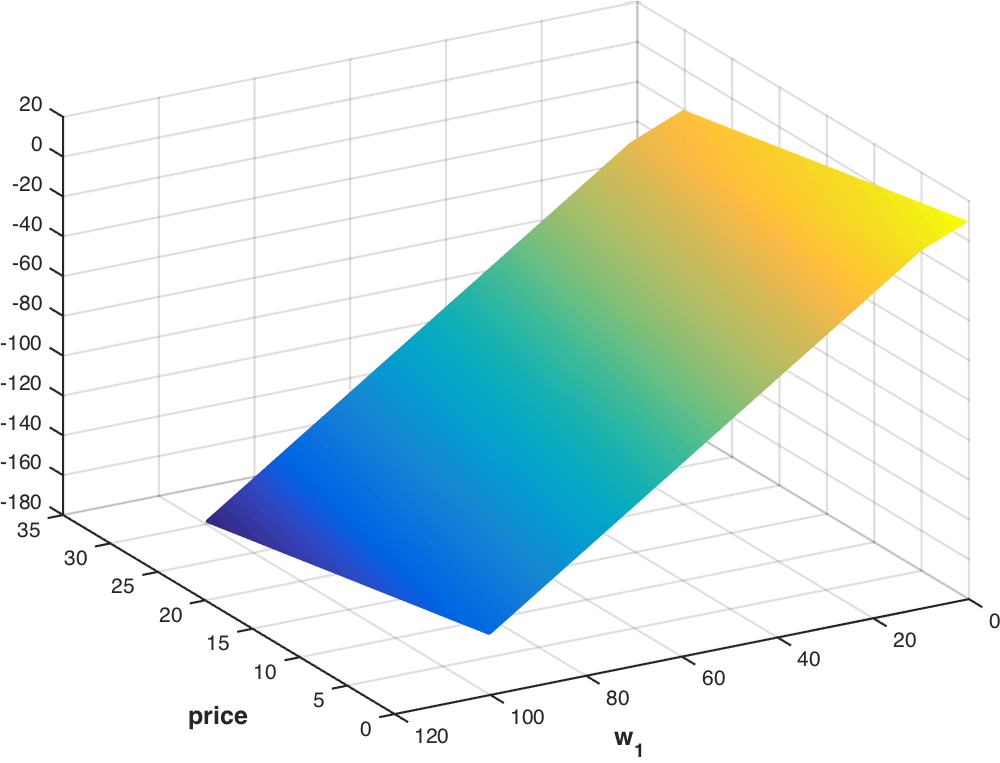
\includegraphics[width=\linewidth, height=0.8\linewidth]{images/opt_execution_w1}
        \caption{$ w_1 \in \left[ 0.0, 100.0 \right]$}
        \label{fig:opt_execution_w1}
        \vspace{1em}
    \end{subfigure}
    
    \begin{subfigure}[b]{0.4\textwidth}    
%        \centering
        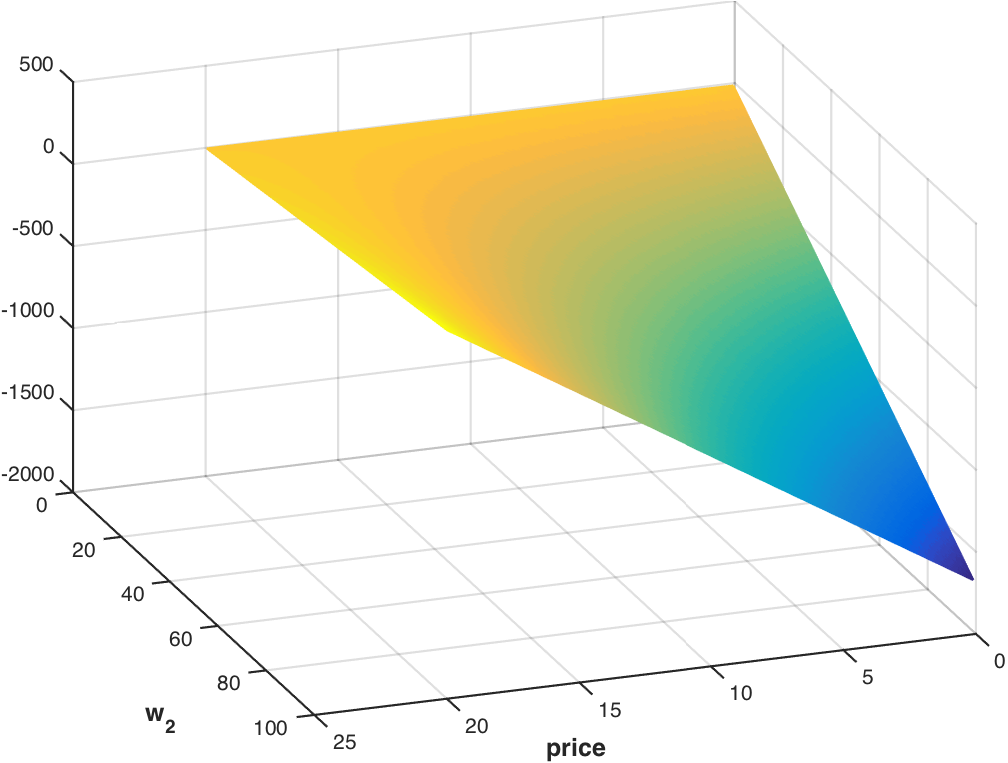
\includegraphics[width=\linewidth, height=0.8\linewidth]{images/opt_execution_w2}
        \caption{$ w_2 \in \left[ 0.0, 100.0 \right]$}
        \label{fig:pt_execution_w2}
    \end{subfigure}  
    \caption{Optimal Execution. $ price \in \left[ 0.0, 20.0 \right]$ is on the x-axis and $ w_1 \in \left[ 0.0, 2.0 \right]$ is on the y-axis. $ price_0 = 10.0, i = 50.0$.}
    \label{fig:pt_execution}
\end{figure}
%------------------------------------------------------------------------------